\chapter{Survey of Message Broker implementations} 
\label{survey-broker}
In previous chapters we first discussed the traditional messaging broker as it
hosts a queue for simply move data between distributed clients without losing
messages or requiring each component to be always available. Regarding to our
second topic, the streaming of big data we saw that a stream is actually an
abstract version of a message broker with special abilities optimized for
further processing events in real-time. 

In the following survey we want to compare implementations of broker system by
mainly comparing the following characteristics---which we already defined in
\todo{ref}---to our reference product Apache Kafka. \todo{ref}

\begin{itemize}
\item Consumption Model 
     \item Delivery Reliability 
         \item Fault Tolerance
\end{itemize}

\section{Implementations}
%\subsection{Traditional Message Broker}

\begin{description}
    \item [Rabbit MQ] \hfill \\
    {
    RabbitMQ is written in Erlang and its source code is released under the
    Mozilla Public License. RabbitMQ supports many messaging protocols, among
    which the most important are STOMP: Streaming Text Oriented Messaging
    Protocol and AMQP: Advanced Messaging Queuing Protocol. Incoming messages
    are placed in a queue whereas this message can further be stored in memory
    or on a disk. The latter model of persistency will underperform when there is 
    a large number of queues which need to access the disk simultaneously.
    \cite{rabbitmq}

    In a RabbitMQ Cluster, queues are created and live in a single node, and all
    nodes know about all the queues. When a node receives a request to a queue
    that is not available in the current node, it routes the request to the node
    that has the queue. To provide high availability (HA), RabbitMQ replicates
    messages between master and a mirrored slave, so the slave can take over if the
    master has died. \cite{wickramarachchi2012andes}

    What RabbitMQ clustering does not do is provide guarantees against message loss.
    When a Rabbit cluster node dies, the messages in queues on that
    node can disappear. This is because RabbitMQ doesn't replicate the contents
    of queues throughout the cluster. They live only on the node that owns the
    queue. \cite{videla2012rabbitmq}
    }
    \item [Active MQ] \hfill \\
    {
    Apache ActiveMQ is an open source message broker written in Java
    together with a full Java Message Service (JMS) client. 

    The messages are stored in a data log (called journal), which consists of
    individual files. When all messages in a data log have been successfully
    consumed, the data log file is marked as being ready to be deleted - or
    archived in a periodical cleanup cycle. Then at intervals the journal can be
    copied to a long term persistence storage (e.g. JDBC). Multiple
    brokers nodes cannot share a journal. Each must be configured with it's own
    journal. The journal cannot be used, however, to recover messages as it does
    not keep an ordered index. So the long term store is used to recover the
    durable subscription. Additionally a separate in-memory reference store
    holds references from those messages residing in the data log to improve
    performance.

    In a clustered long term persistence setup, Apache Zookeeper
    is used to pick a master from a set of broker nodes configured to replicate
    a LevelDB Store. Then synchronizes all slave LevelDB Stores with the master
    keeps them up to date by replicating all updates from the master. 

    ActiveMQ will preserve the order of messages sent by a single producer to
    all consumers on a topic. If there is a single consumer on a queue then the
    order of messages sent by a single producer will be preserved as well.
    However due to multi-threading and asynchronous processing, the messages
    from different producers could arrive in different consumers in different
    orders. 
    \cite{activemq}
    }
\end{description}


%\subsection{Streaming Broker}
\begin{description}
    \item [Amazon SQS] \hfill \\
    {
    Amazon Simple Queuing Service is a cloud service which offers a simple
    message queue to move data between distributed systems. SQS guarantees
    reliability by redelivering Messages in case of failure. If a message is
    successfully processed by a consumer it will be deleted out of the queue.
    Amazon SQS does not guarantee a strict ordering of messages. All messages
    are stored redundantly on multiple servers and in multiple data center.
    \cite{amazonSQS} \cite{amazonSQSFaq} 

    SQS as itself can not provide a publish subscribe behaviour as in typical
    message brokers. But in combination with the Amazon Simple  Notification
    Service (SNS) it is possible to create topics which are linked to SQS queues
    where consumers can register itself and only receive message from a specific
    topic. \cite{amazonSqsPubSub}
     }
    \item [Amazon Kinesis] \hfill \\
    { 
    Amazon Kinesis is a cloud service for streaming event
    data for further processing which is very similar to Apache Kafka. Producer
    applications push data continuously to the Kinesis broker where the messages
    are keept for 24 hours in memory. Kinesis provides ordering of records, as
    well as the ability to read and/or replay records in the same order to
    multiple Amazon Kinesis Applications.
    \cite{amazonKinesis} \cite{amazonKinesisFAQ} 
    
   \begin{figure}[H]
     \centering
     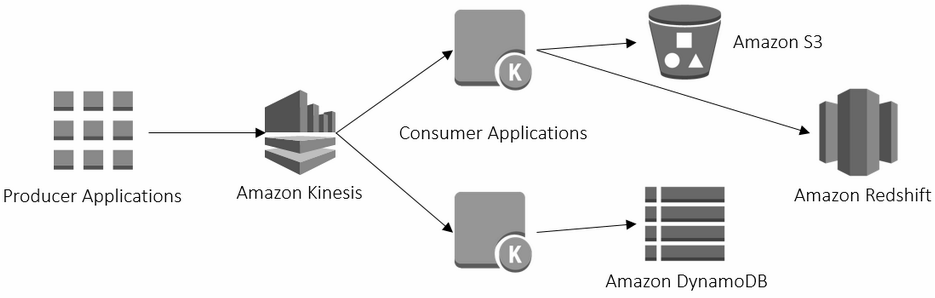
\includegraphics[width=0.7\textwidth]{images/amazon-kinesis.png}
         \caption{Amazon Kinesis aggregates events and interacts with other AWS
         Cloud services \cite{amazonKinesis}}
        \label{fig:amazon-kinesis}
    \end{figure}
    }
    \item [Scribe] \hfill \\
    { Push based, no pub-sub, static configuration}
    \item [Kastrell] \hfill \\
    {no clustering; no pub-sub}
    \item [Apache Flume] \hfill \\
    {Flume is a distributed service specialized on being a reliable way of
    getting event data into HDFS \todo{gls}. The typical deployment consists
    of a number of logical nodes, arranged into three tiers. The first tier
    is the agent tier. Agent nodes are typically installed on the machines
    that generate the data and are the initial point of contact with Flume.
    They forward data to the next tier of collector nodes, which aggregate the
    separate data flows and forward them to the final storage tier. Flume is
    push based and does not support public-subscribe semantics. \cite{apacheflumeDoc}
    \begin{figure}[H]
     \centering
     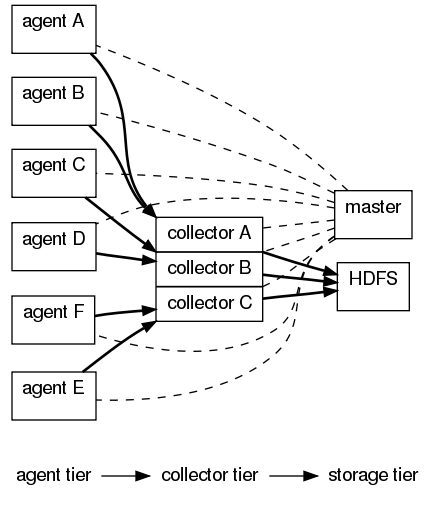
\includegraphics[width=0.4\textwidth]{images/flume-architecture.png}
     \caption{Apache Flume general architecture \cite{apacheflumeDoc}} 
        \label{fig:flume-architecture}
    \end{figure}

    }
\end{description}

\begin{landscape}
\section{Overview}

\begin{table}[h]
    \begin{tabular}{|p{3cm}|p{3cm}|p{3cm}|p{3cm}|p{3cm}|p{3cm}|p{3cm}|}
        \hline
                                  & \textbf{ActiveMQ}                     & {\textbf{Apache Kafka}}         & \textbf{Apache Flume}  & \textbf{Amazon Kinesis} & \textbf{Amazon SQS}                                     & \textbf{RabbitMQ}          \\ \hline
        \textbf{Maker}                     & Apache Foundation            &LinkedIn                      & Cloudera               & Amazon                  & Amazon                                                  & Pivolat Software           \\ \hline
        \textbf{Written in}                & Java                         & Scala                         & Java                   & -                       & -                                                       & Erlang                     \\ \hline
        \textbf{License}                   & Apache License 2.0           & Apache License 2.0            & Apache License 2.0     &                         &                                                         & Mozilla Public Licence     \\ \hline
        \textbf{Type}                      & Traditional Message Broker   & Message Broker / Event Stream & Event Stream           & Event Stream (Cloud)    & Messaging Queue Service (Cloud)                         & Traditional Message Broker \\ \hline
        \textbf{Standards            }     & JMS / AMQP                   &                               &                        &                         &                                                         & AMQP                       \\ \hline
        \textbf{Ordering-Guarantee}        &                              &     \multicolumn{1}{c|}{X}     &                        & \multicolumn{1}{c|}{X}  & no                                                      &                            \\ \hline
        \textbf{Delivery-Semantic}         & At Least Once, Exactly Once  & At Least Once                 & At Least Once          & At Least Once           & Exactly once                                            &                            \\ \hline
        \textbf{Public-Subscribe}          & \multicolumn{1}{c|}{X}       & \multicolumn{1}{c|}{X}                                                 & \multicolumn{1}{c|}{}  & \multicolumn{1}{c|}{X}  & X* & \multicolumn{1}{c|}{X}     \\ \hline
        \textbf{Pull-Consumption}          &                              &                                                   &                        &                         &                                                         &                            \\ \hline
        \textbf{Push-Consumption}          &                              &  \multicolumn{1}{c|}{X}                                                   & \multicolumn{1}{c|}{X} &                         &                                                         &                            \\ \hline
        \textbf{Longterm-Persistence}      & \multicolumn{1}{c|}{X}       &  \multicolumn{1}{c|}{X}                                                & \multicolumn{1}{c|}{X} & \multicolumn{1}{c|}{X}  &                                                         &                            \\ \hline
        \textbf{Streamprocessing Clients}  &                              &  \multicolumn{1}{c|}{X}                                                 &                        & \multicolumn{1}{c|}{}   &                                                         &                            \\ \hline
        \textbf{Storage Clients}           &                              &  \multicolumn{1}{c|}{X}                                               & \multicolumn{1}{c|}{X} &                         &                                                         &                            \\ \hline
        \textbf{Clustering}                &                              &  \multicolumn{1}{c|}{X}                                                    &                        & \multicolumn{1}{c|}{X}  &                                                         &                            \\ \hline
    \end{tabular}
\end{table}

\end{landscape}

\section{Conclusion}
\todo[inline]{Welches System passt für welchen Anwendungsfall und welche nicht
(Gründe)}






